% 2014 全国卷Ⅰ理科第 12 题：小正方形边长为 1 的三视图。
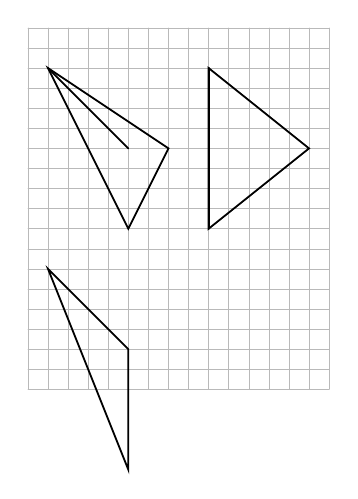
\begin{tikzpicture}[x=2.55mm,y=2.55mm,line cap=round]
  \draw[step=1,gray!55,line width=.18pt] (0,0) grid (15,18);
  % 左上投影：两条斜边从同一顶点出发。
  \draw[line width=.65pt] (1,16)--(7,12)--(5,8)--cycle;
  \draw[line width=.65pt] (1,16)--(5,12);
  % 右上投影：指向右侧的三角形投影。
  \draw[line width=.65pt] (9,16)--(14,12)--(9,8)--cycle;
  \draw[line width=.65pt] (9,16)--(9,8);
  % 左下投影：斜线三角形。
  \draw[line width=.65pt] (1,6)--(5,2)--(5,-4)--cycle;
\end{tikzpicture}
